\subsection*{23 april 2014}
\label{sec:meeting-23-apr}

Aanwezig: \textit{Herman, Patrick, Hylke, Johan}

\begin{description}
\item[Tekenen overeenkomsten] De overeenkomsten zijn ondertekend.

\item[Plan van aanpak] 

\item[Ontwikkelproces] Johan vertelt dat de ontwikkelmethode \textit{SCRUM} gebruikt zal worden. In principe hebben we vrijheid om het project in te delen zoals dat ons handig lijkt. Hij wil globaal op de hoogte gehouden worden van de vorderingen. Johan zal zich een halve tot een dag in de week bezig houden met het project. Hij zal zich niet bezighouden met de documenten en presentaties die bij de TU Delft aangeleverd moeten worden.

Ideaal gezien zou het systeem opgedeeld worden in (onafhankelijke) componenten Johan zou graag zien dat er een verdeling wordt gemaakt van ``managers'' op deze componenten.

\item[Wekelijkse meeting plannen voor voortgang, doelen en taken] De dagelijkse standups staan in de agenda (waar we nog toegang toe krijgen). Wat Johan betreft hebben we dan geen wekelijkse meetings nodig.

\item[Ontwikkelomgeving en versiebeheer] Johan laat de Visual Studio Online omgeving en Visual Studio zien.

\item[Testen en \mylaps X2 introductie] Johan laat de \mylaps X2 Manager zien.

\item[Architectuur] Johan vertelt hoe andere applicaties van Emando globaal zijn opgezet. Er zijn verschillende lagen die elk verantwoordelijk zijn voor een bepaald aspect van de applicatie. Deze lagen kunnen onafhankelijk van elkaar ontwikkeld en getest worden.

\begin{itemize}
  \item De presentatielaag bevat de User Interface.
  \item De servicelaag bevat bijvoorbeeld de API.
  \item De businesslaag bevat alle functionaliteit voor het verwerken van data.
  \item De datalaag bevat databases etc.
\end{itemize}

\end{description}

\subsection*{1 mei 2014}
\label{sec:meeting-1-mei}

Aanwezig: \textit{Herman, Patrick, Johan}\\
Locatie: aan bureau's

\begin{figure}
\centering
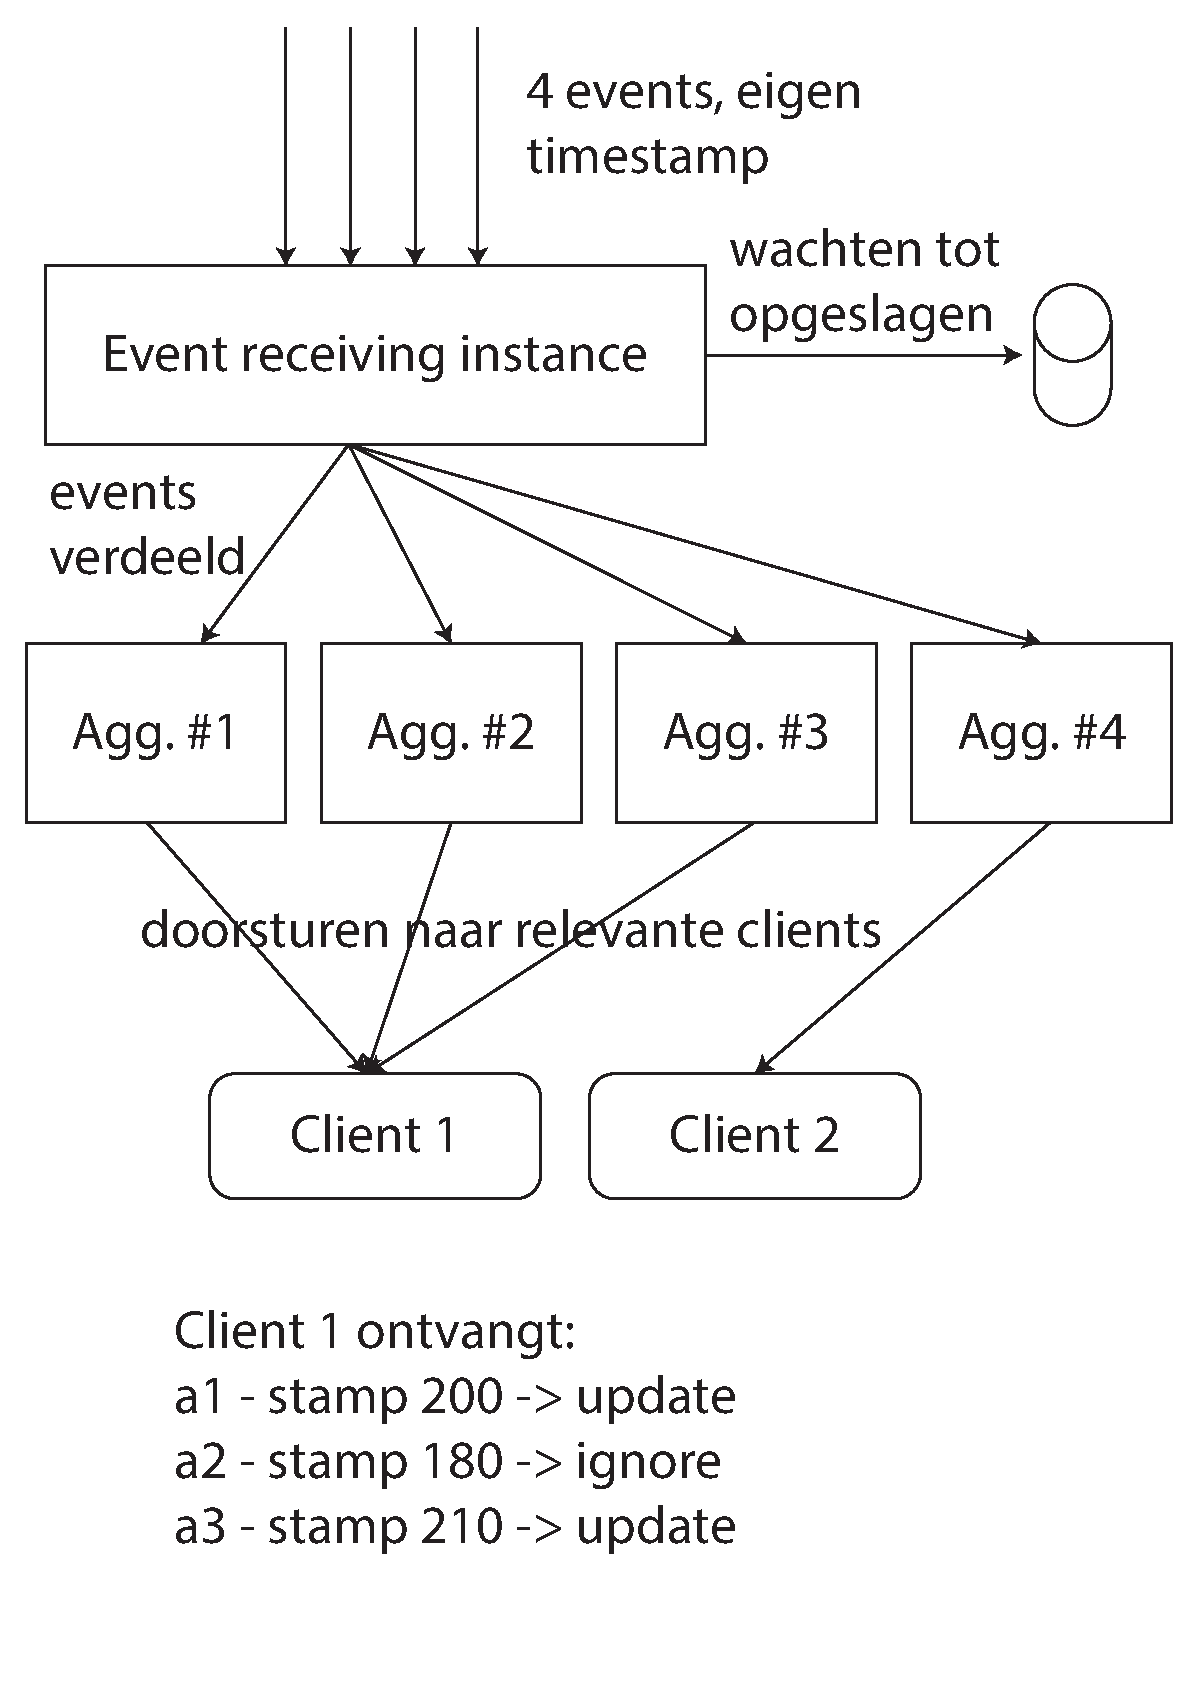
\includegraphics[width=0.4\textwidth]{style/images/meeting1mei}
\caption{Flow bij het binnenkomen van nieuwe Passings}
\label{fig:not1mei}
\end{figure}

\begin{description}
\item[Aggregaties] Aggregaties worden opgeslagen met de timestamp van de laatste Passing die meegenomen is in de berekening. Het doen van de aggregaties kan dus verdeeld worden over meerdere instances, want de laatste Passing die binnenkwam heeft altijd de nieuwste data. De client gebruikt alleen aggregaties met een nieuwe timestamp dan die hij al had. Dit is geschetst en staat in figuur~\ref{fig:not1mei}.

Opslaan van aggregaties kan in Azure Table Store. De partitie id is de (virtuele) groep en de row is de user. De kolommen zijn de verschillende aggregaties. Wanneer er voor een user een nieuwe aggregatie is gedaan worden de normale groepen geupdate en ook de virtuele groepen zoals de aggregatie specifiek voor passings op de specifieke baan waar de laatste passing van binnenkwam.

\begin{table}[h!]
\begin{tabular}{lccccc}
\centering
\textbf{group  } & \textbf{ person } & langste training & snelste ronde & percentage rust/runs \\
\textbf{g1     } & \textbf{ p1     } & 30               & 31            & 10 \\
\textbf{g2     } & \textbf{ p1     } & 31               & 32            & 30 \\
\textbf{g2     } & \textbf{ p2     } & 30               & 30            & 24 \\
\textbf{g3     } & \textbf{ p2     } & 50               & 34            & 60 \\
\textbf{b1     } & \textbf{ p1     } & 32               & 32            & 10 \\
\textbf{b2     } & \textbf{ p1     } & 35               & 30            & 80 \\
\end{tabular}
\label{tab:tablestore} 
\caption{Idee voor aggregatie tabel}
\end{table}

\end{description}